\subsubsection{Giao diện Admin - Quản lý công việc}

Trang quản lý công việc được thiết kế để hiển thị danh sách toàn bộ các công việc hiện có trong hệ thống, phục vụ việc quản lý, chỉnh sửa hoặc xóa công việc. Dữ liệu cũng được lấy từ Backend thông qua API theo cơ chế phân trang tương tự như các phần trước, giúp tối ưu hóa hiệu suất và hiển thị mượt mà, đặc biệt khi số lượng công việc lớn.

\begin{figure}[H]
    \centering
    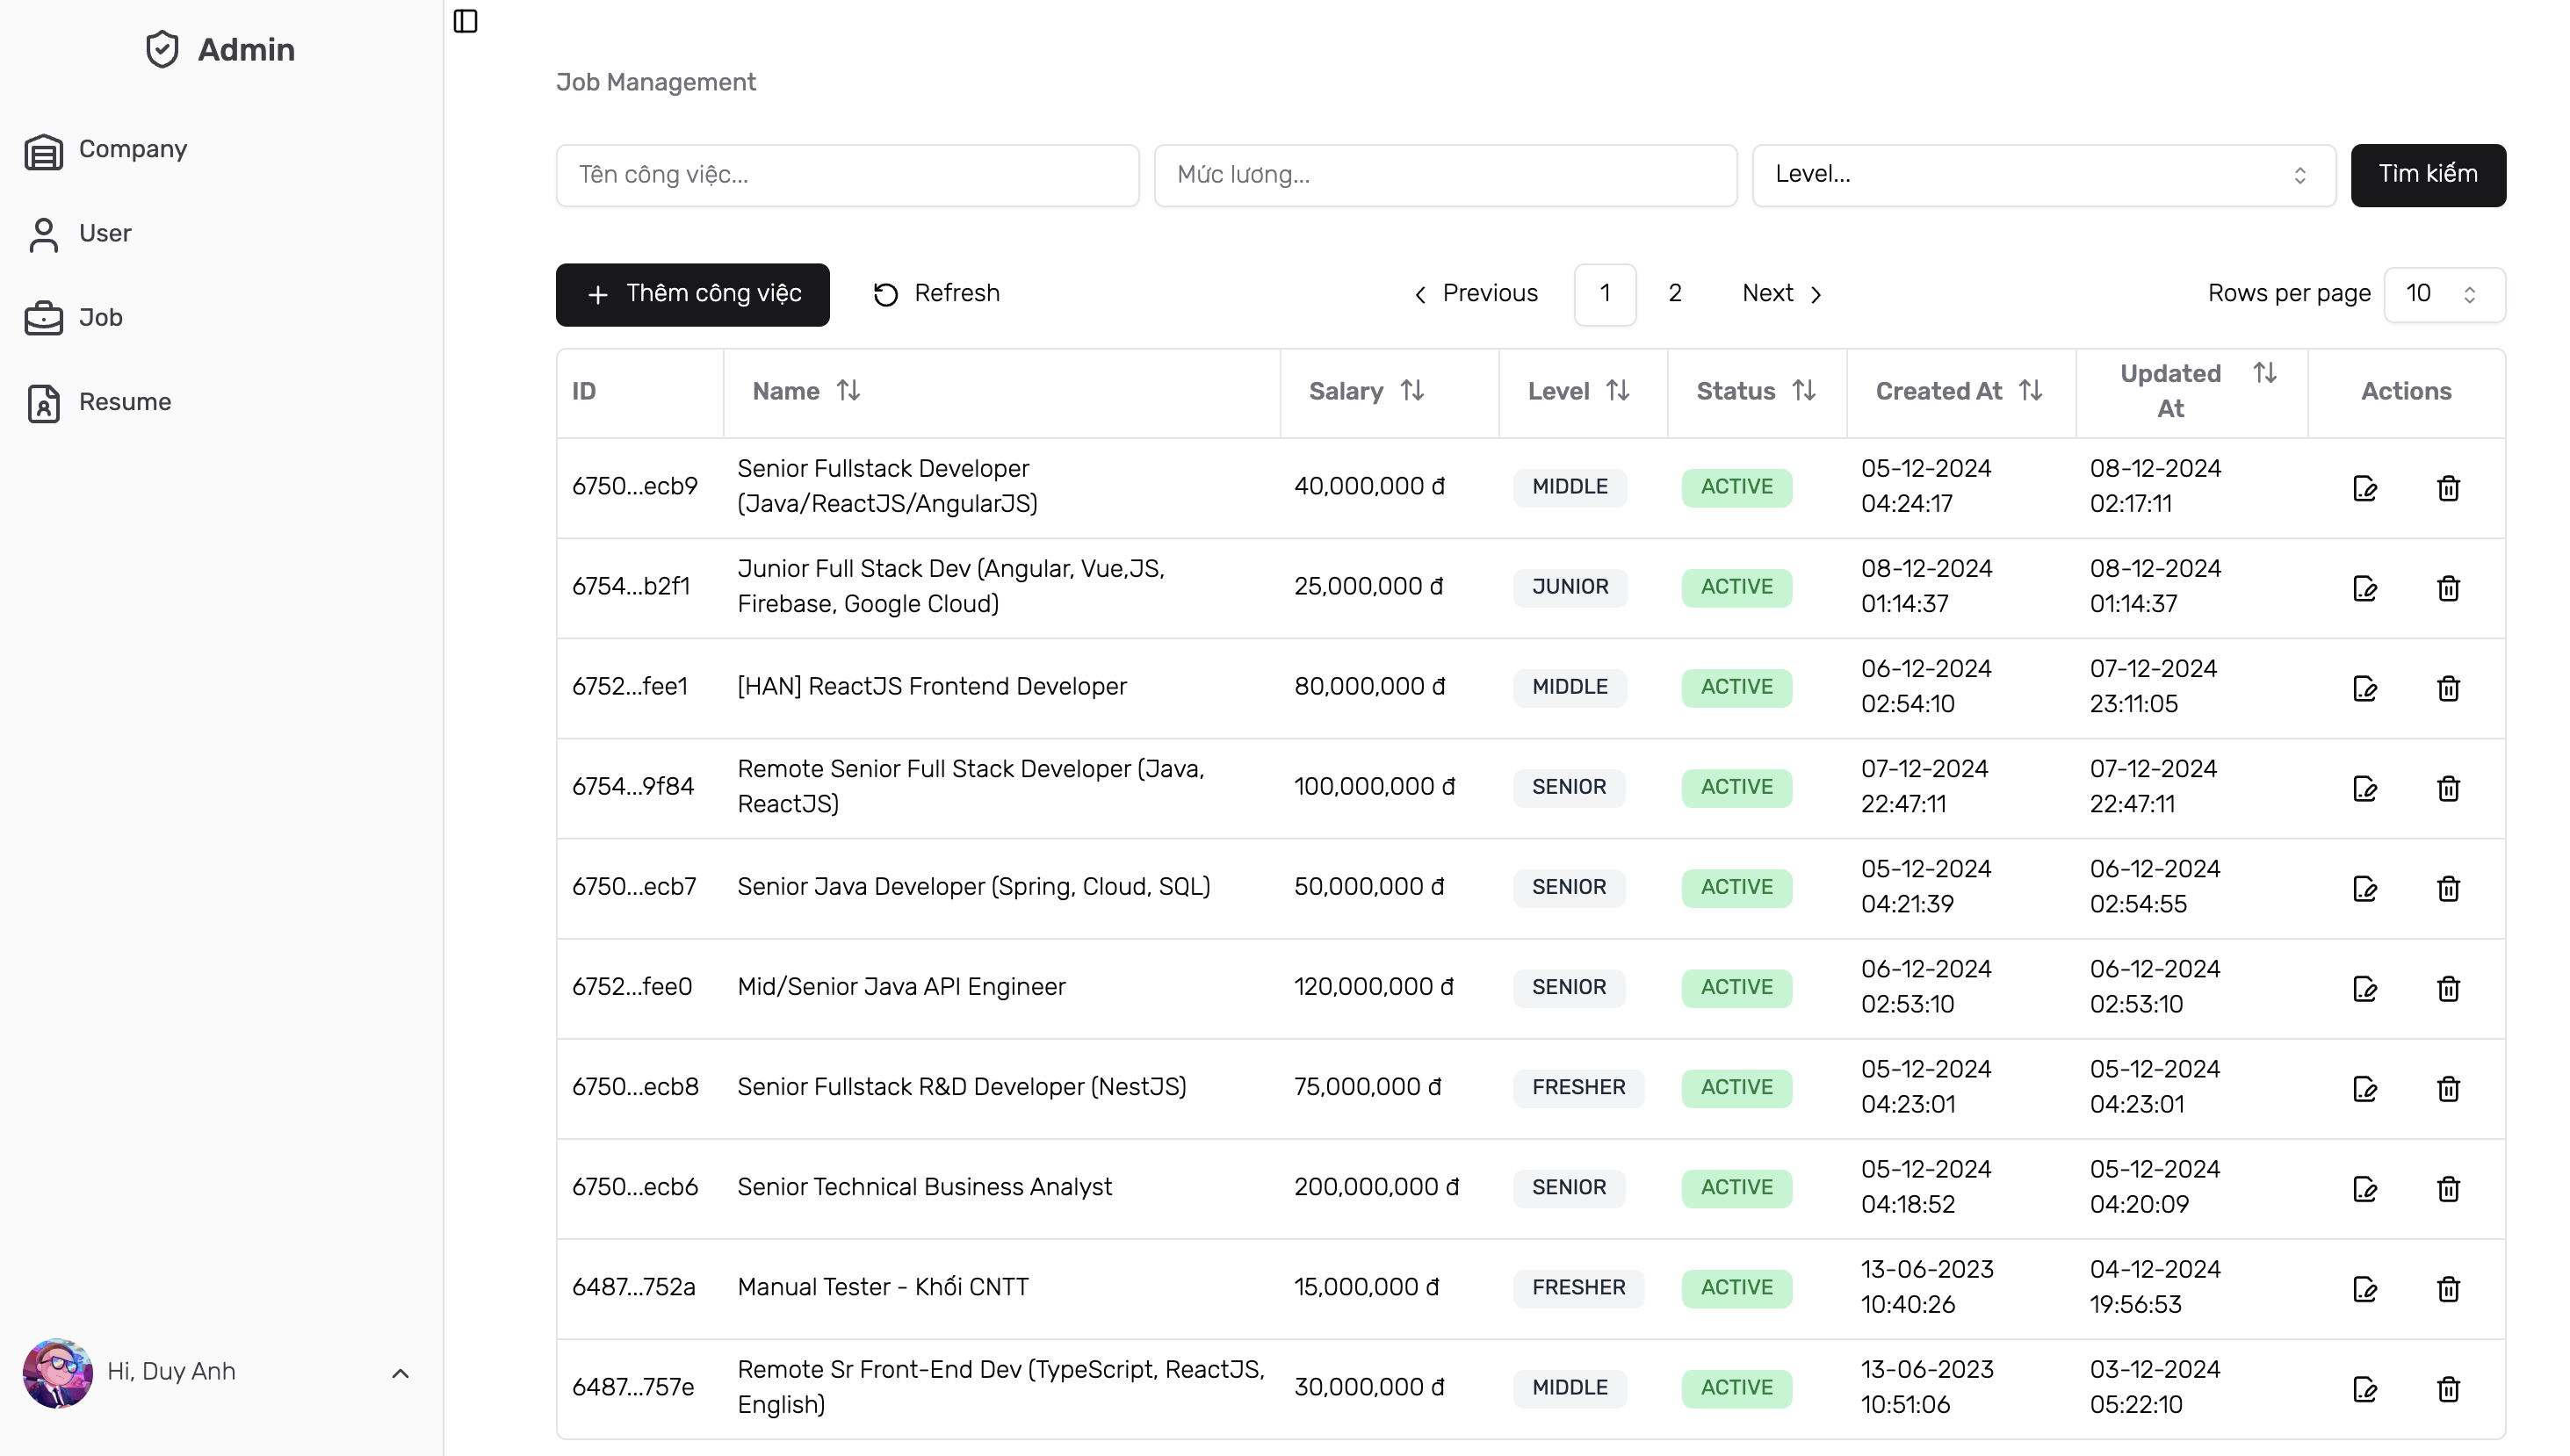
\includegraphics[width=\linewidth]{DBMS-Application/Images/admin-job.png}
    \caption{Trang quản lý công việc - Danh sách các công việc trong hệ thống}
    \label{fig:enter-label}
\end{figure}

Quản trị viên cũng có thể tìm kiếm và lọc ra các công ty theo \textbf{Tên}, \textbf{Mức lương} và \textbf{Level} như sau:

\begin{figure}[H]
    \centering
    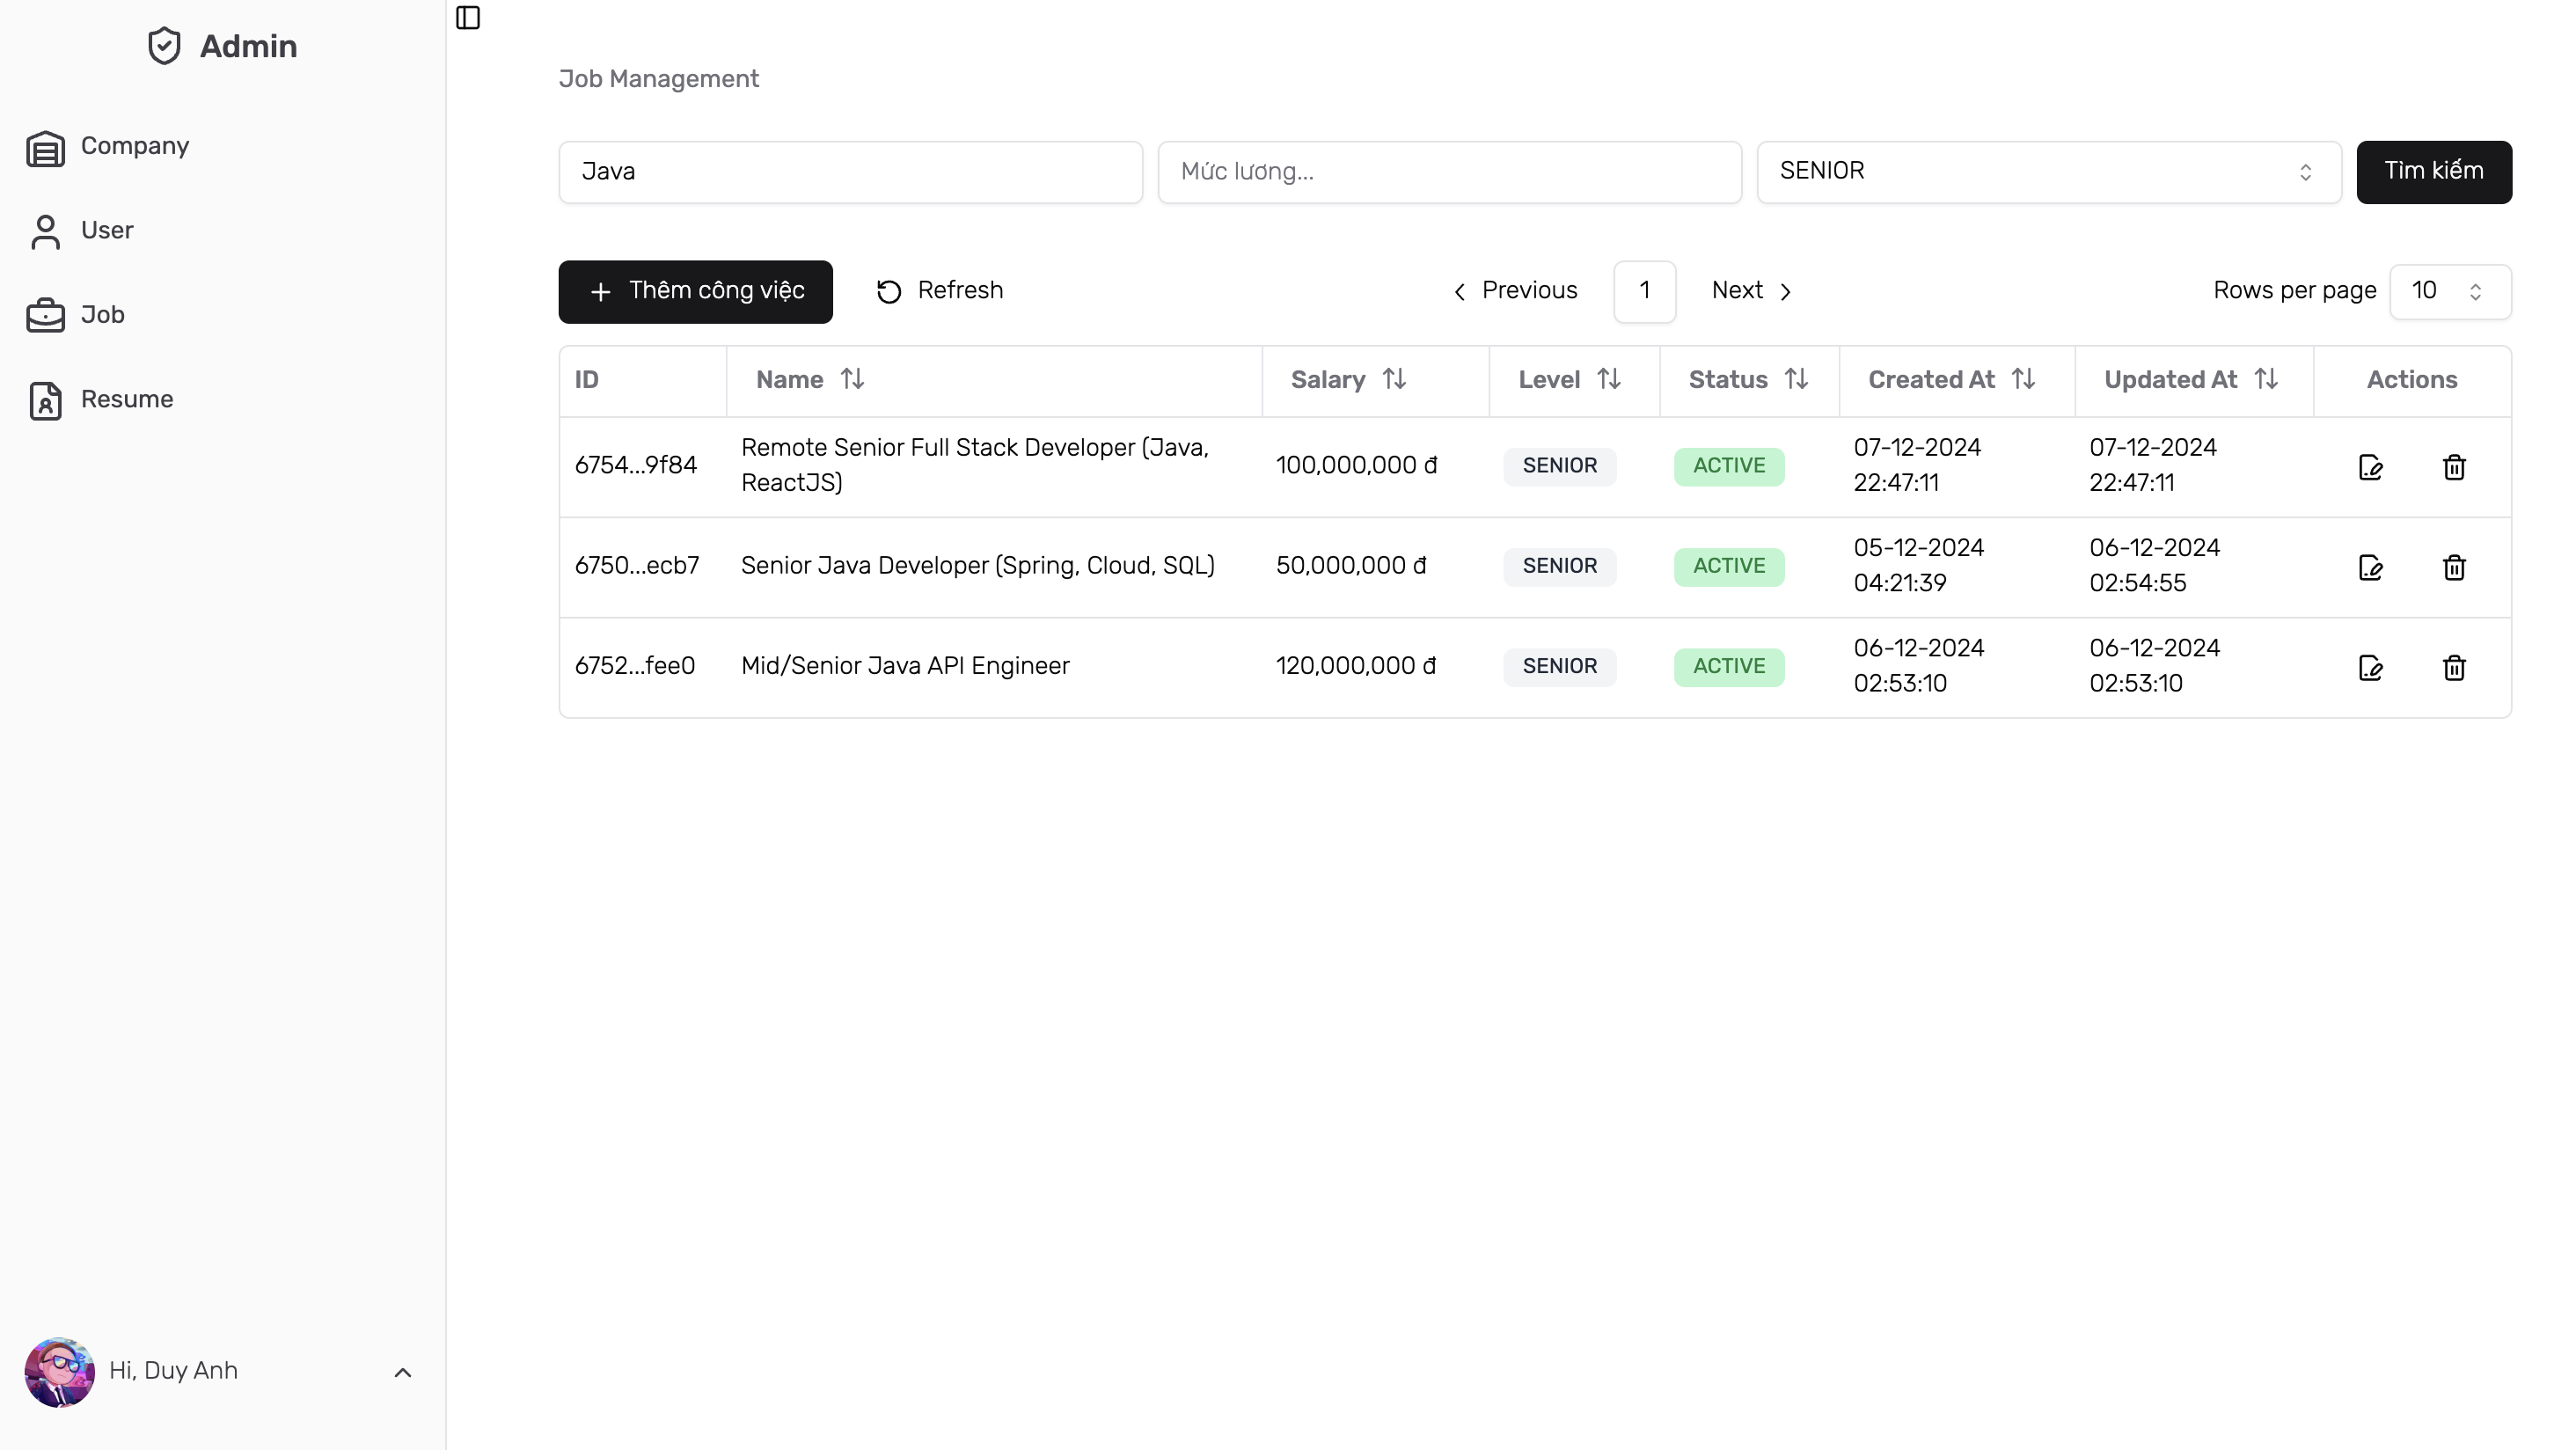
\includegraphics[width=\linewidth]{DBMS-Application/Images/admin-job-filter.png}
    \caption{Trang quản lý công việc - Danh sách công việc lọc theo điều kiện}
    \label{fig:enter-label}
\end{figure}

Truy vấn sử dụng: \textbf{Query with single/composite condition}\\

Bên cạnh đó, quản trị viên cũng có thể thêm công việc mới, bằng cách điền các thông tin cần thiết vào giao diện dưới đây. Sau đó, hệ thống sẽ gửi thông tin này đến cơ sở dữ liệu để thực hiện việc thêm document mới vào collection \textbf{jobs}.

\begin{figure}[H]
    \centering
    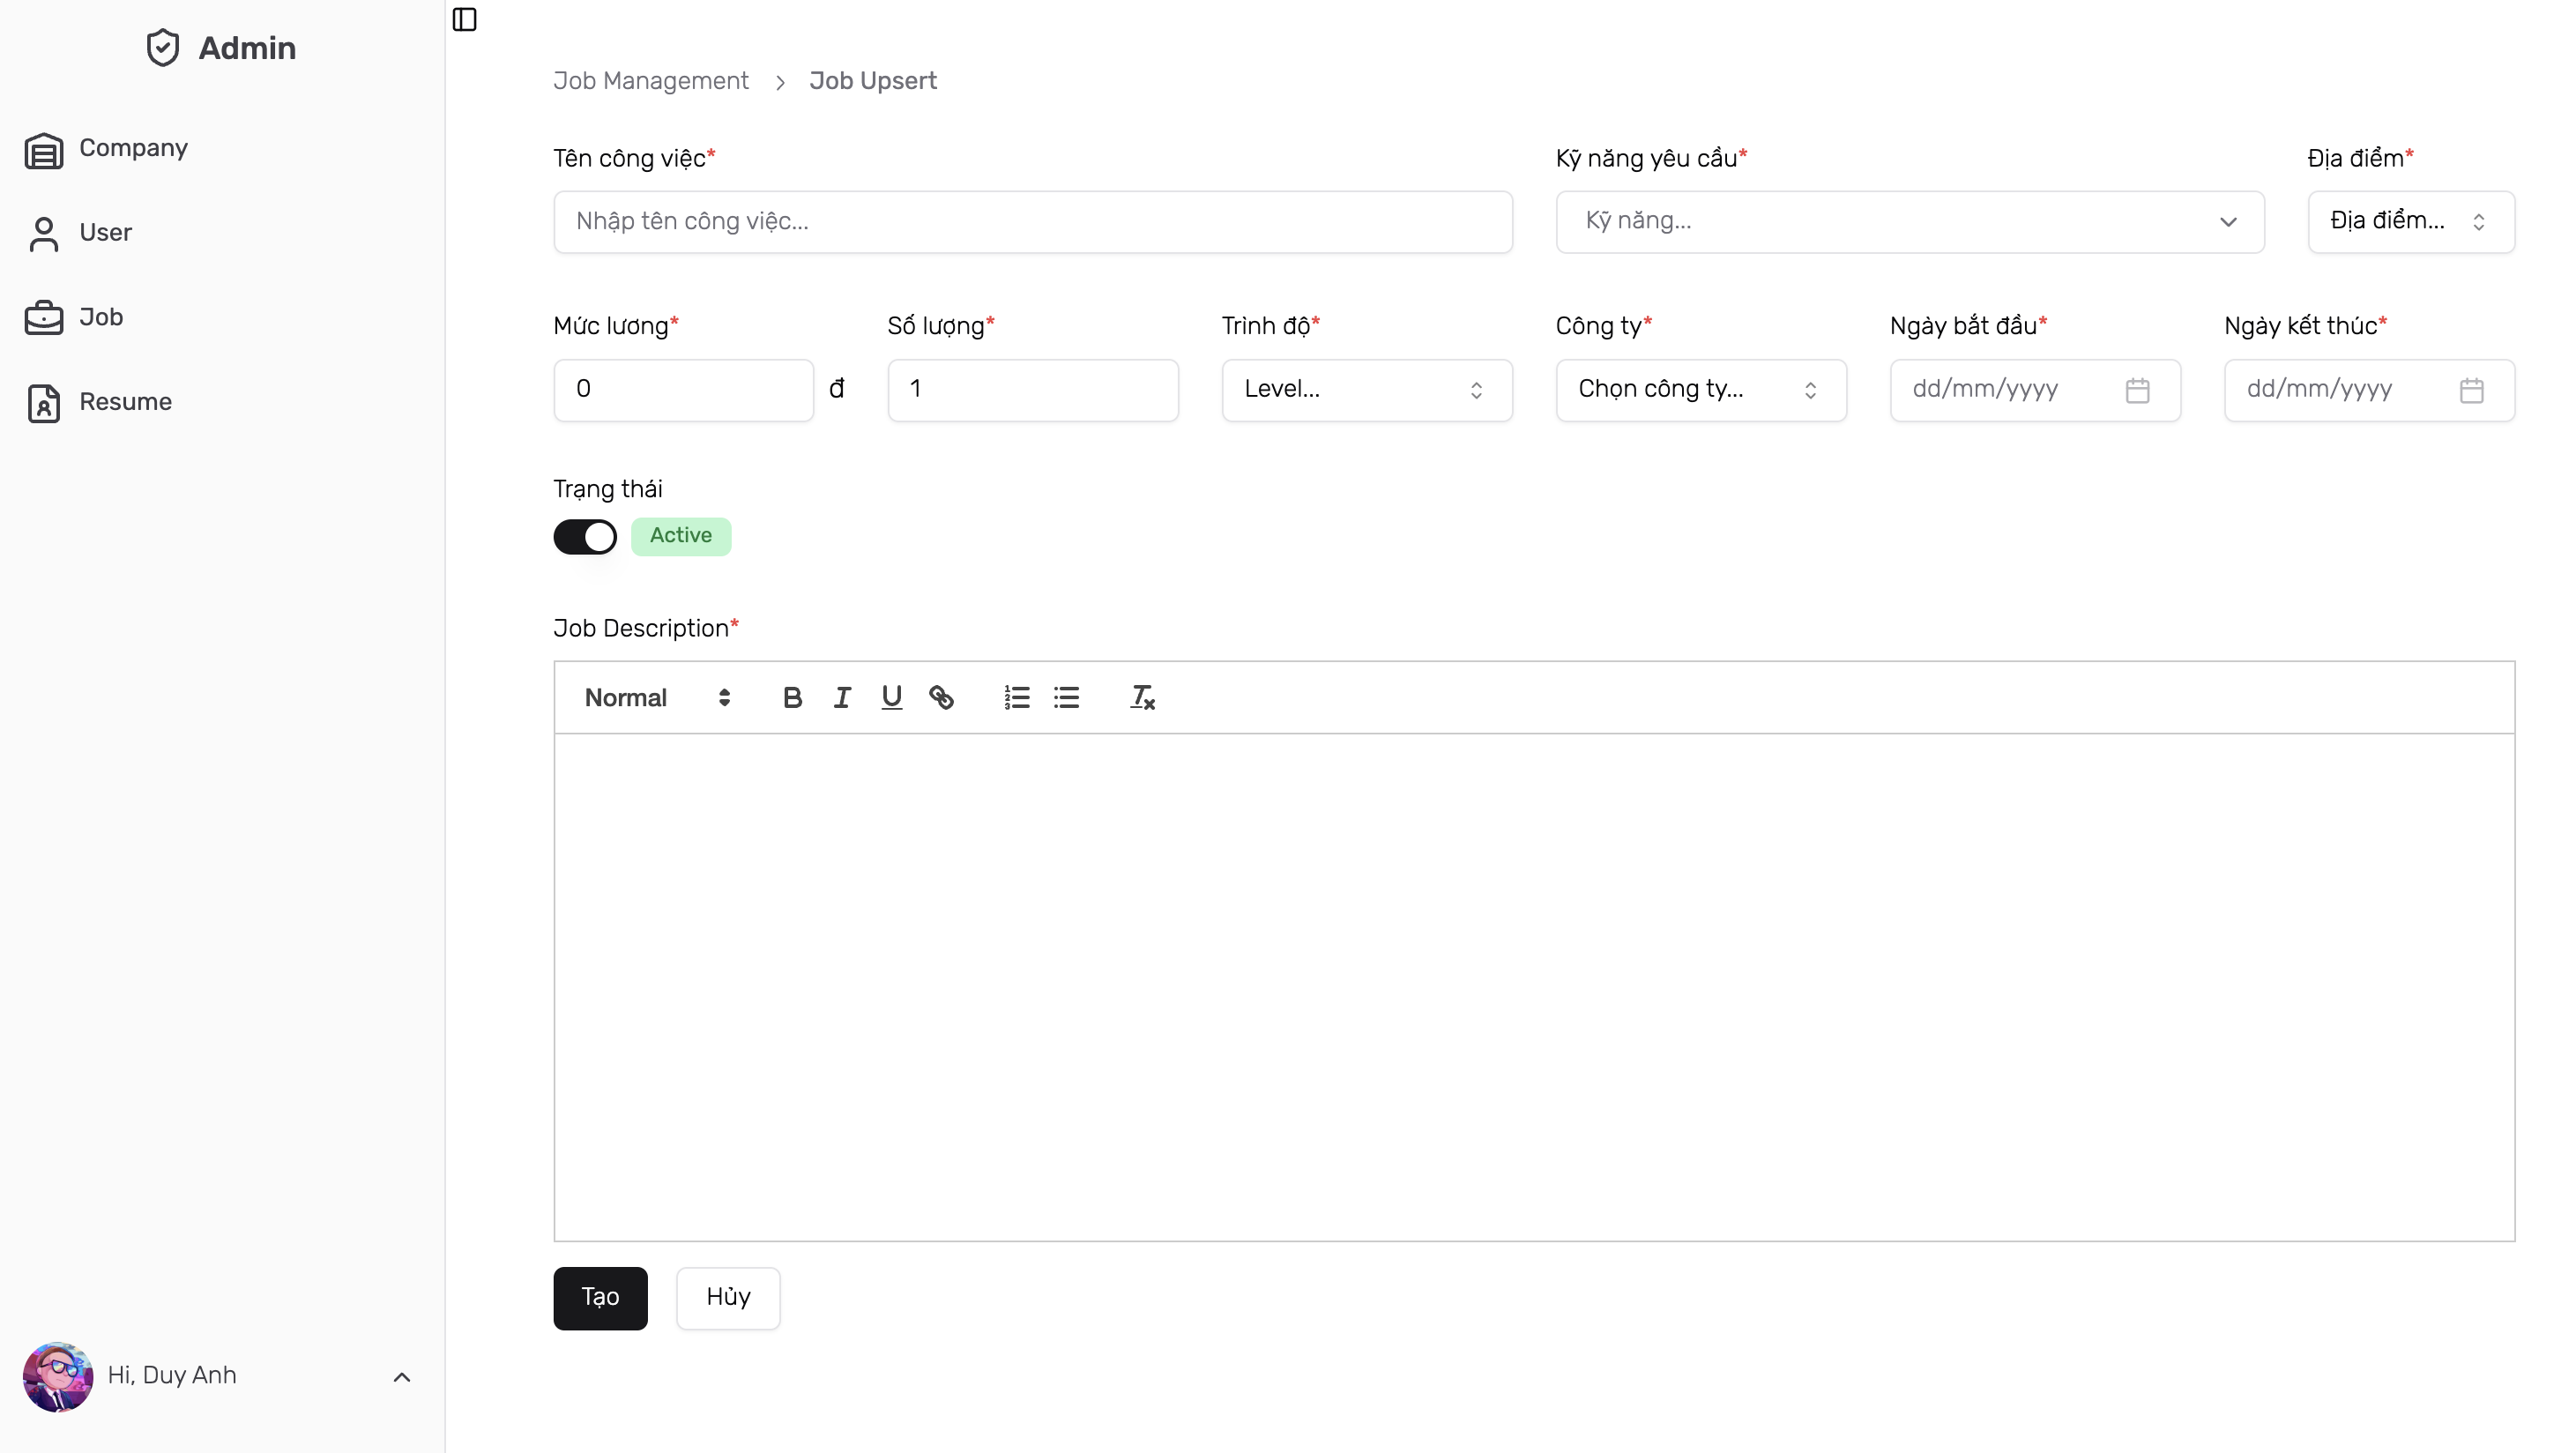
\includegraphics[width=\linewidth]{DBMS-Application/Images/create-job.png}
    \caption{Trang quản lý công việc - Thêm công việc mới}
    \label{fig:enter-label}
\end{figure}

Truy vấn sử dụng: \textbf{Insert}

\begin{lstlisting}
async create(createJobDto: CreateJobDto) {
    const job = {
      ...createJobDto,
      createdAt: new Date(),
      updatedAt: new Date(),
    };

    const result = await this.db.collection('jobs').insertOne(job); // Insert cong viec moi vao collection 'jobs'
    return { _id: result.insertedId, createdAt: job.createdAt };
}
\end{lstlisting}

Quản trị viên cũng có thể chọn một công việc để chỉnh sửa/cập nhật thông tin. Khi đó, dựa vào \texttt{\_id}, hệ thống sẽ truy vấn cơ sở dữ liệu để lấy ra công việc đó (\textbf{query with single condition}) và hiển thị lên giao diện. Lúc này, quản trị viên có thể tiến hành sửa lại các thông tin đó và khi hoàn tất, Front-end sẽ gửi yêu cầu qua API với phương thức HTTP \textbf{PATCH} để hệ thống tiến hành cập nhật lại thông tin cho công việc đó trong cơ sở dữ liệu.

\begin{figure}[H]
    \centering
    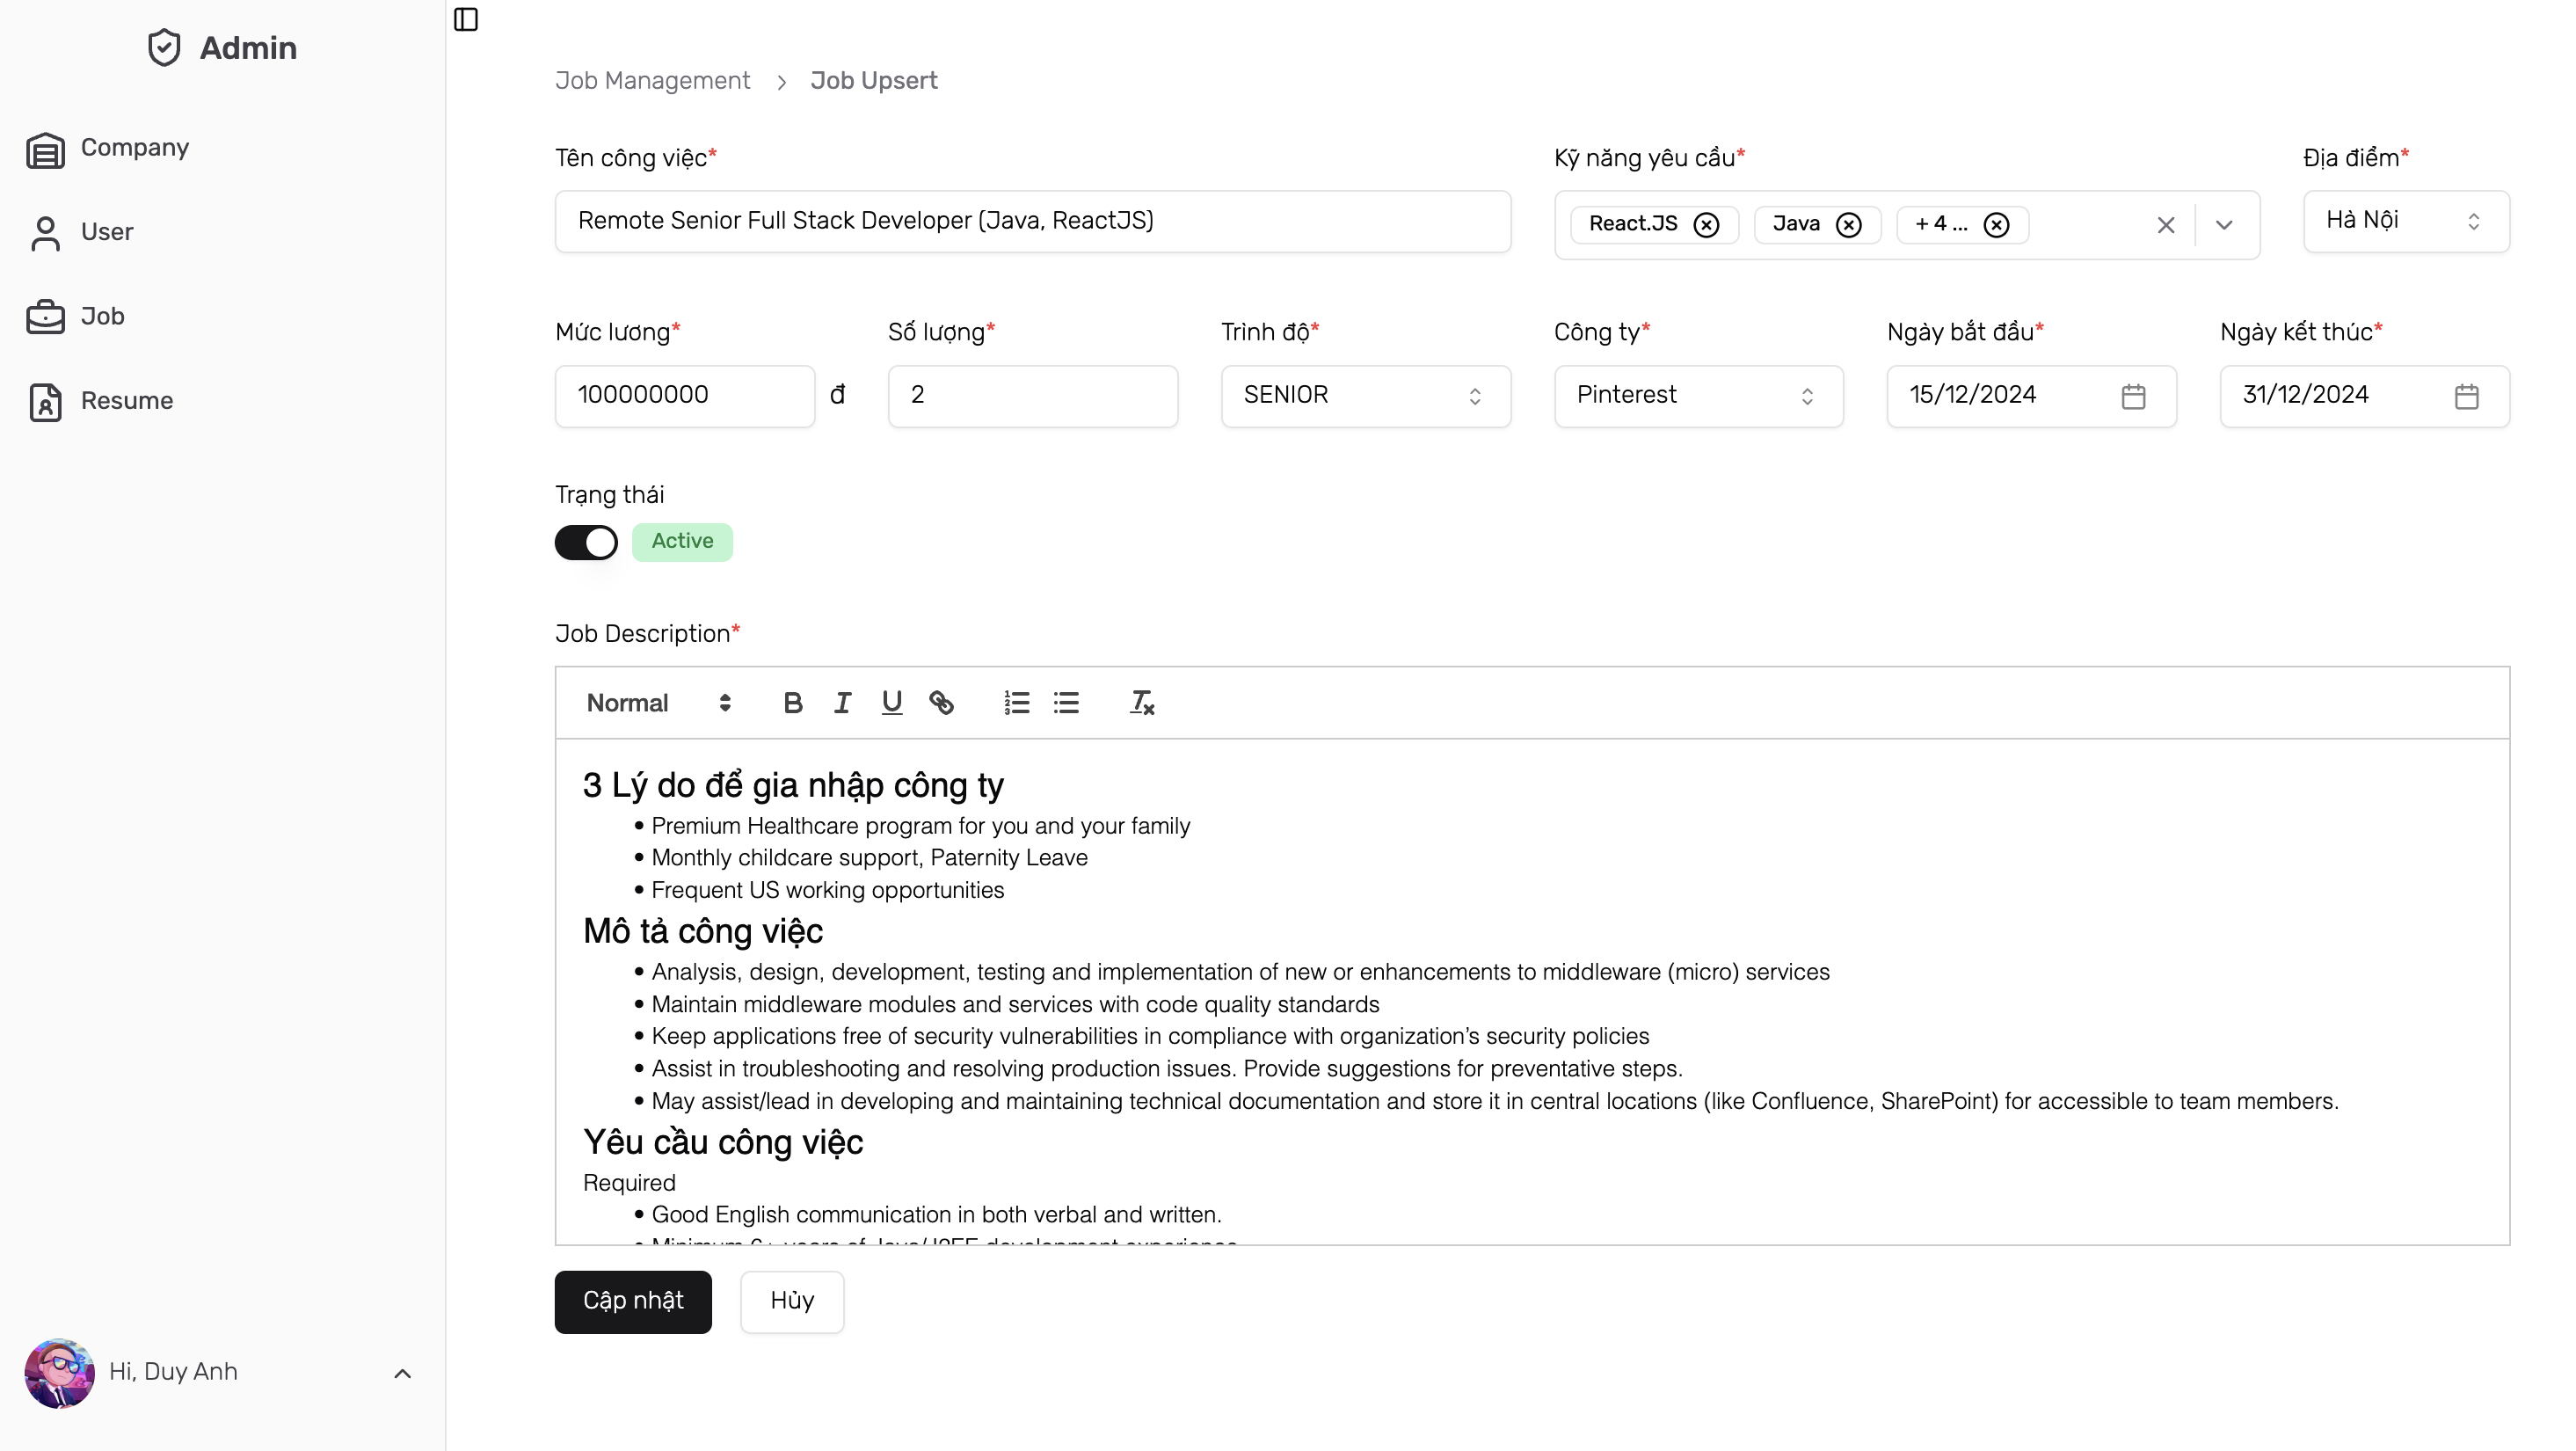
\includegraphics[width=\linewidth]{DBMS-Application/Images/update-job.png}
    \caption{Trang quản lý công việc - Cập nhật thông tin cho một công việc cụ thể}
    \label{fig:enter-label}
\end{figure}

Truy vấn sử dụng: \textbf{Update}

\begin{lstlisting}
const result = await this.db.collection('jobs').updateOne(
  { _id: new ObjectId(id) },
  {
    $set: {
      ...updateJobDto,
      updatedAt: new Date(),
    },
  },
);
\end{lstlisting}

Cuối cùng, quản trị viên có thể chọn một công việc để xoá khỏi hệ thống. Khi đó, một popup sẽ hiện lên để xác nhận với quản trị viên về việc xoá công ty đã chọn ra khỏi cơ sở dữ liệu

\begin{figure}[H]
    \centering
    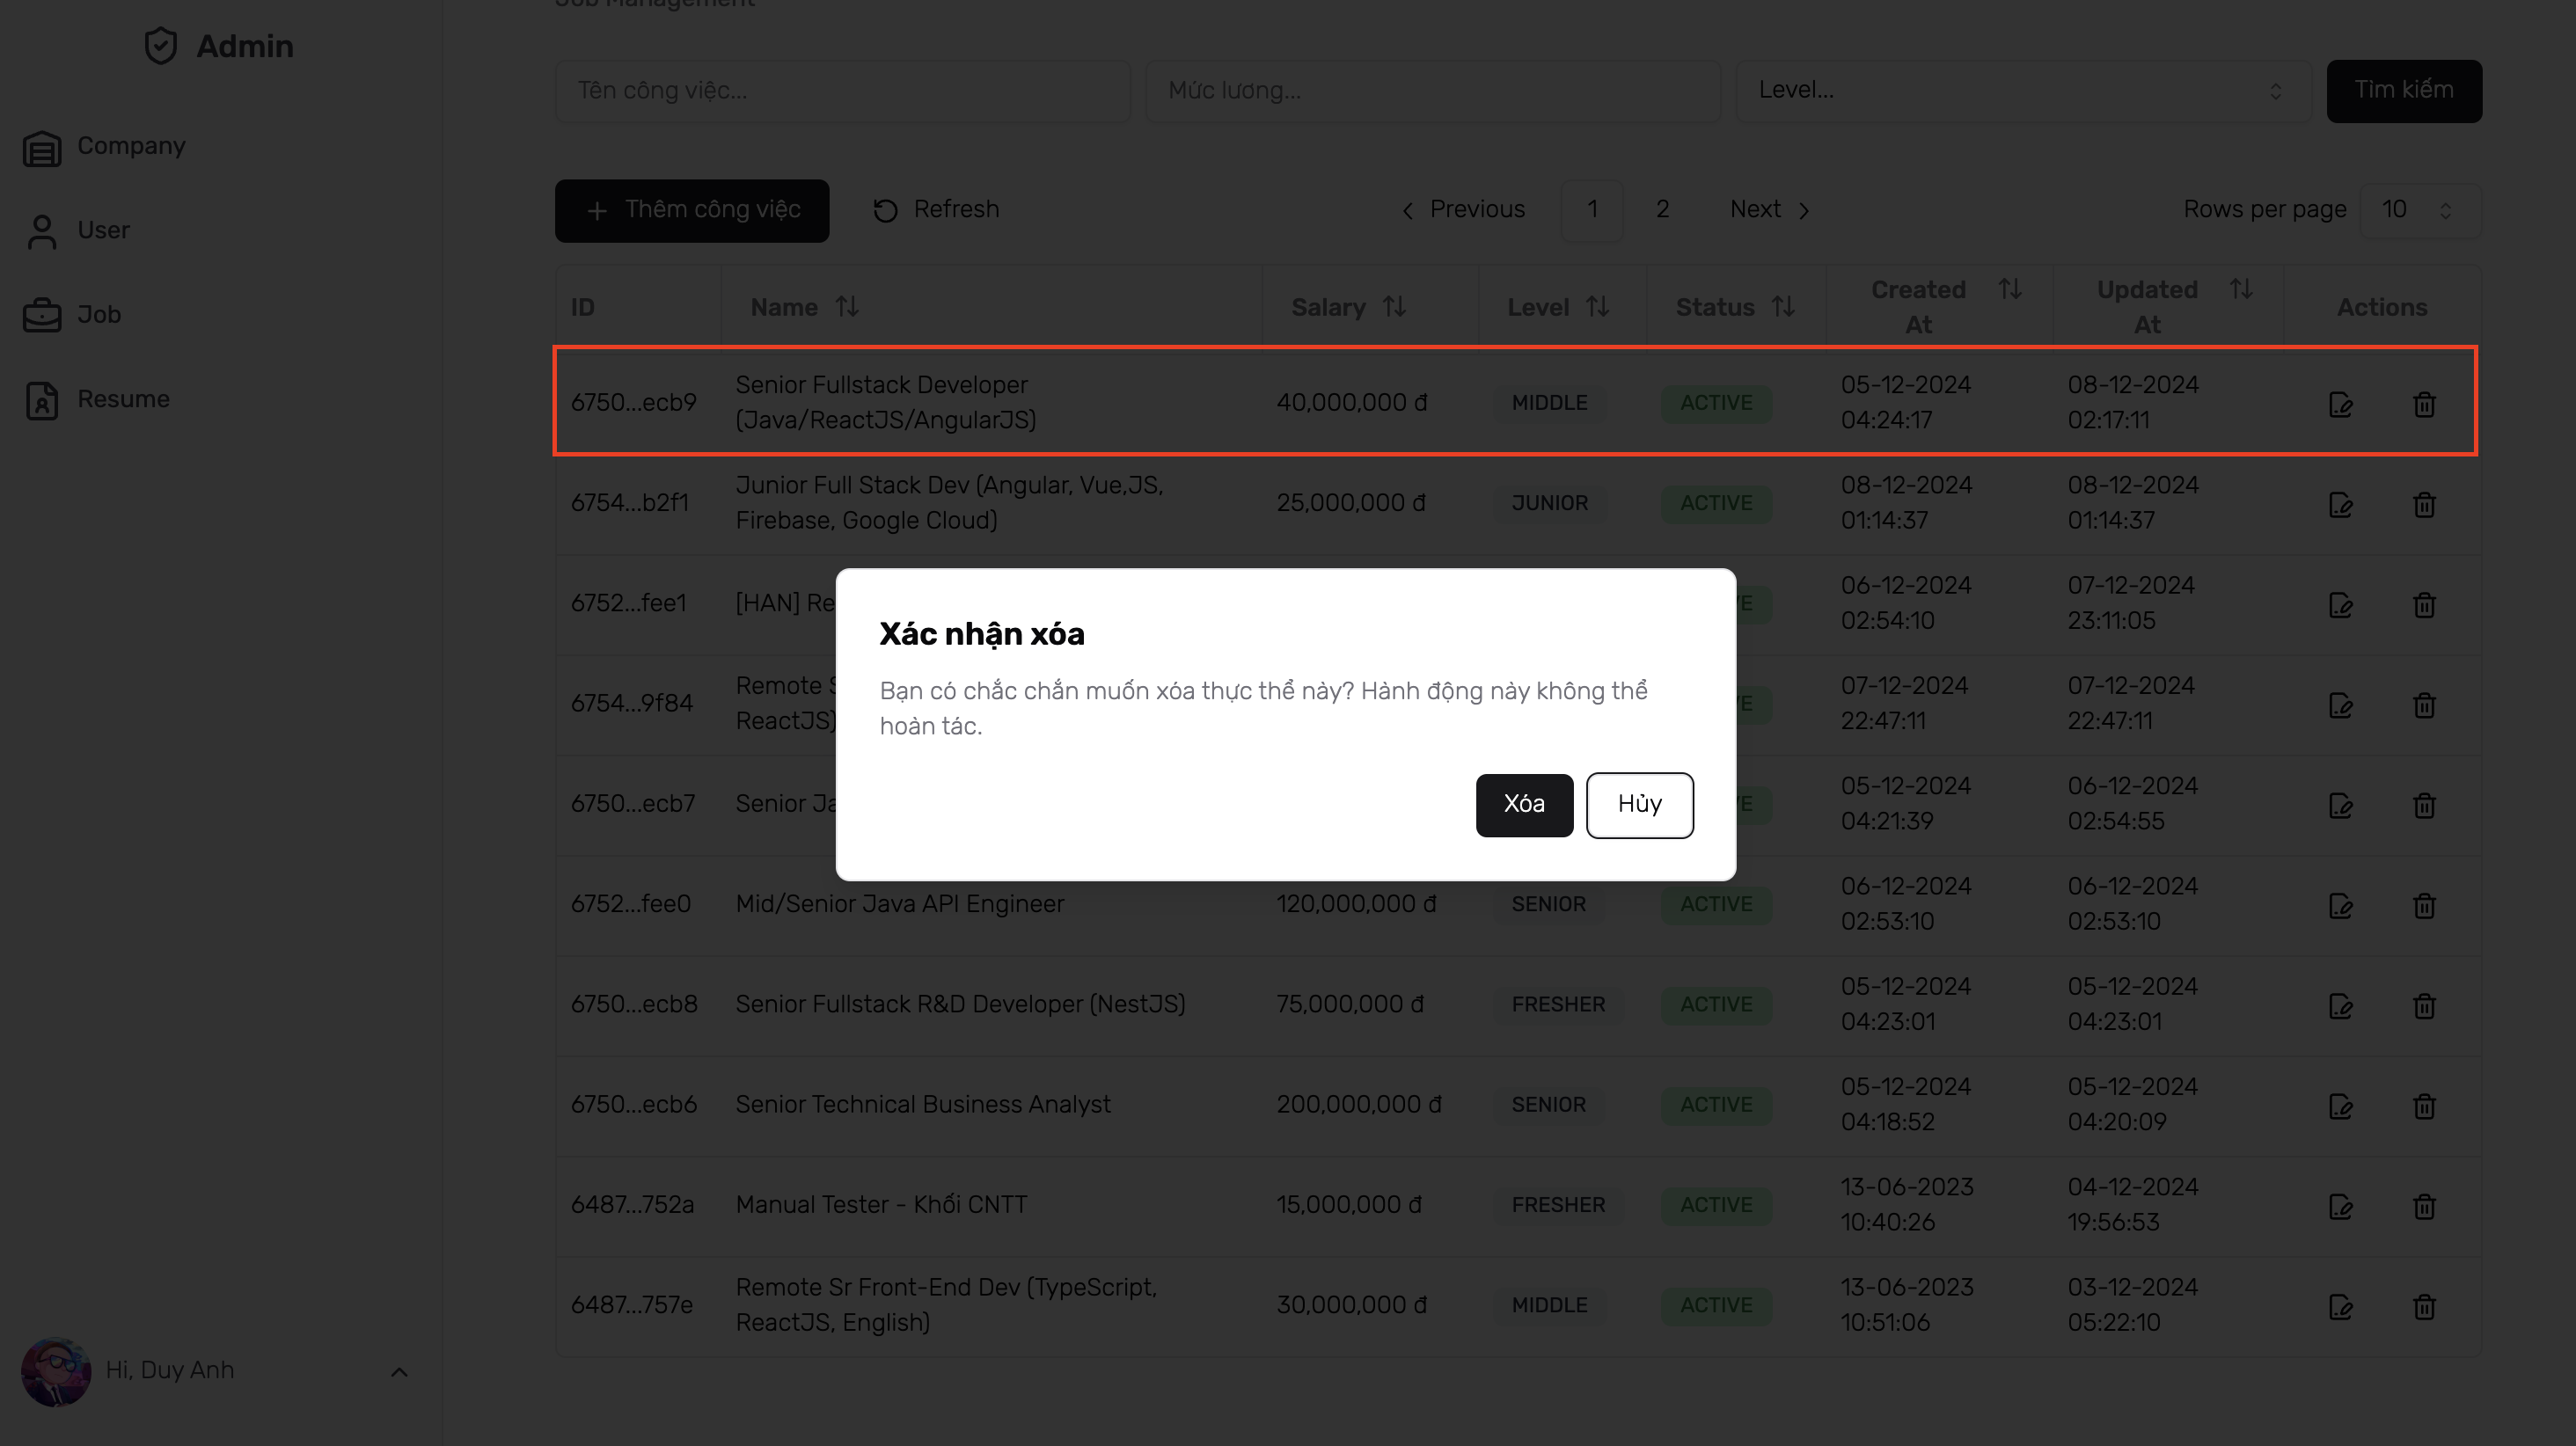
\includegraphics[width=\linewidth]{DBMS-Application/Images/delete-job.png}
    \caption{Trang quản lý công việc - Xác nhận xoá công việc chỉ định khỏi hệ thống}
    \label{fig:enter-label}
\end{figure}

Khi quản trị viên xác nhận, Back-end gửi truy vấn đến cơ sở dữ liệu để tìm theo \texttt{\_id} và xoá công việc đó ra khỏi cơ sở dữ liệu. Khi đó, giao diện người dùng sẽ được cập nhật lại.\\

\begin{figure}[H]
    \centering
    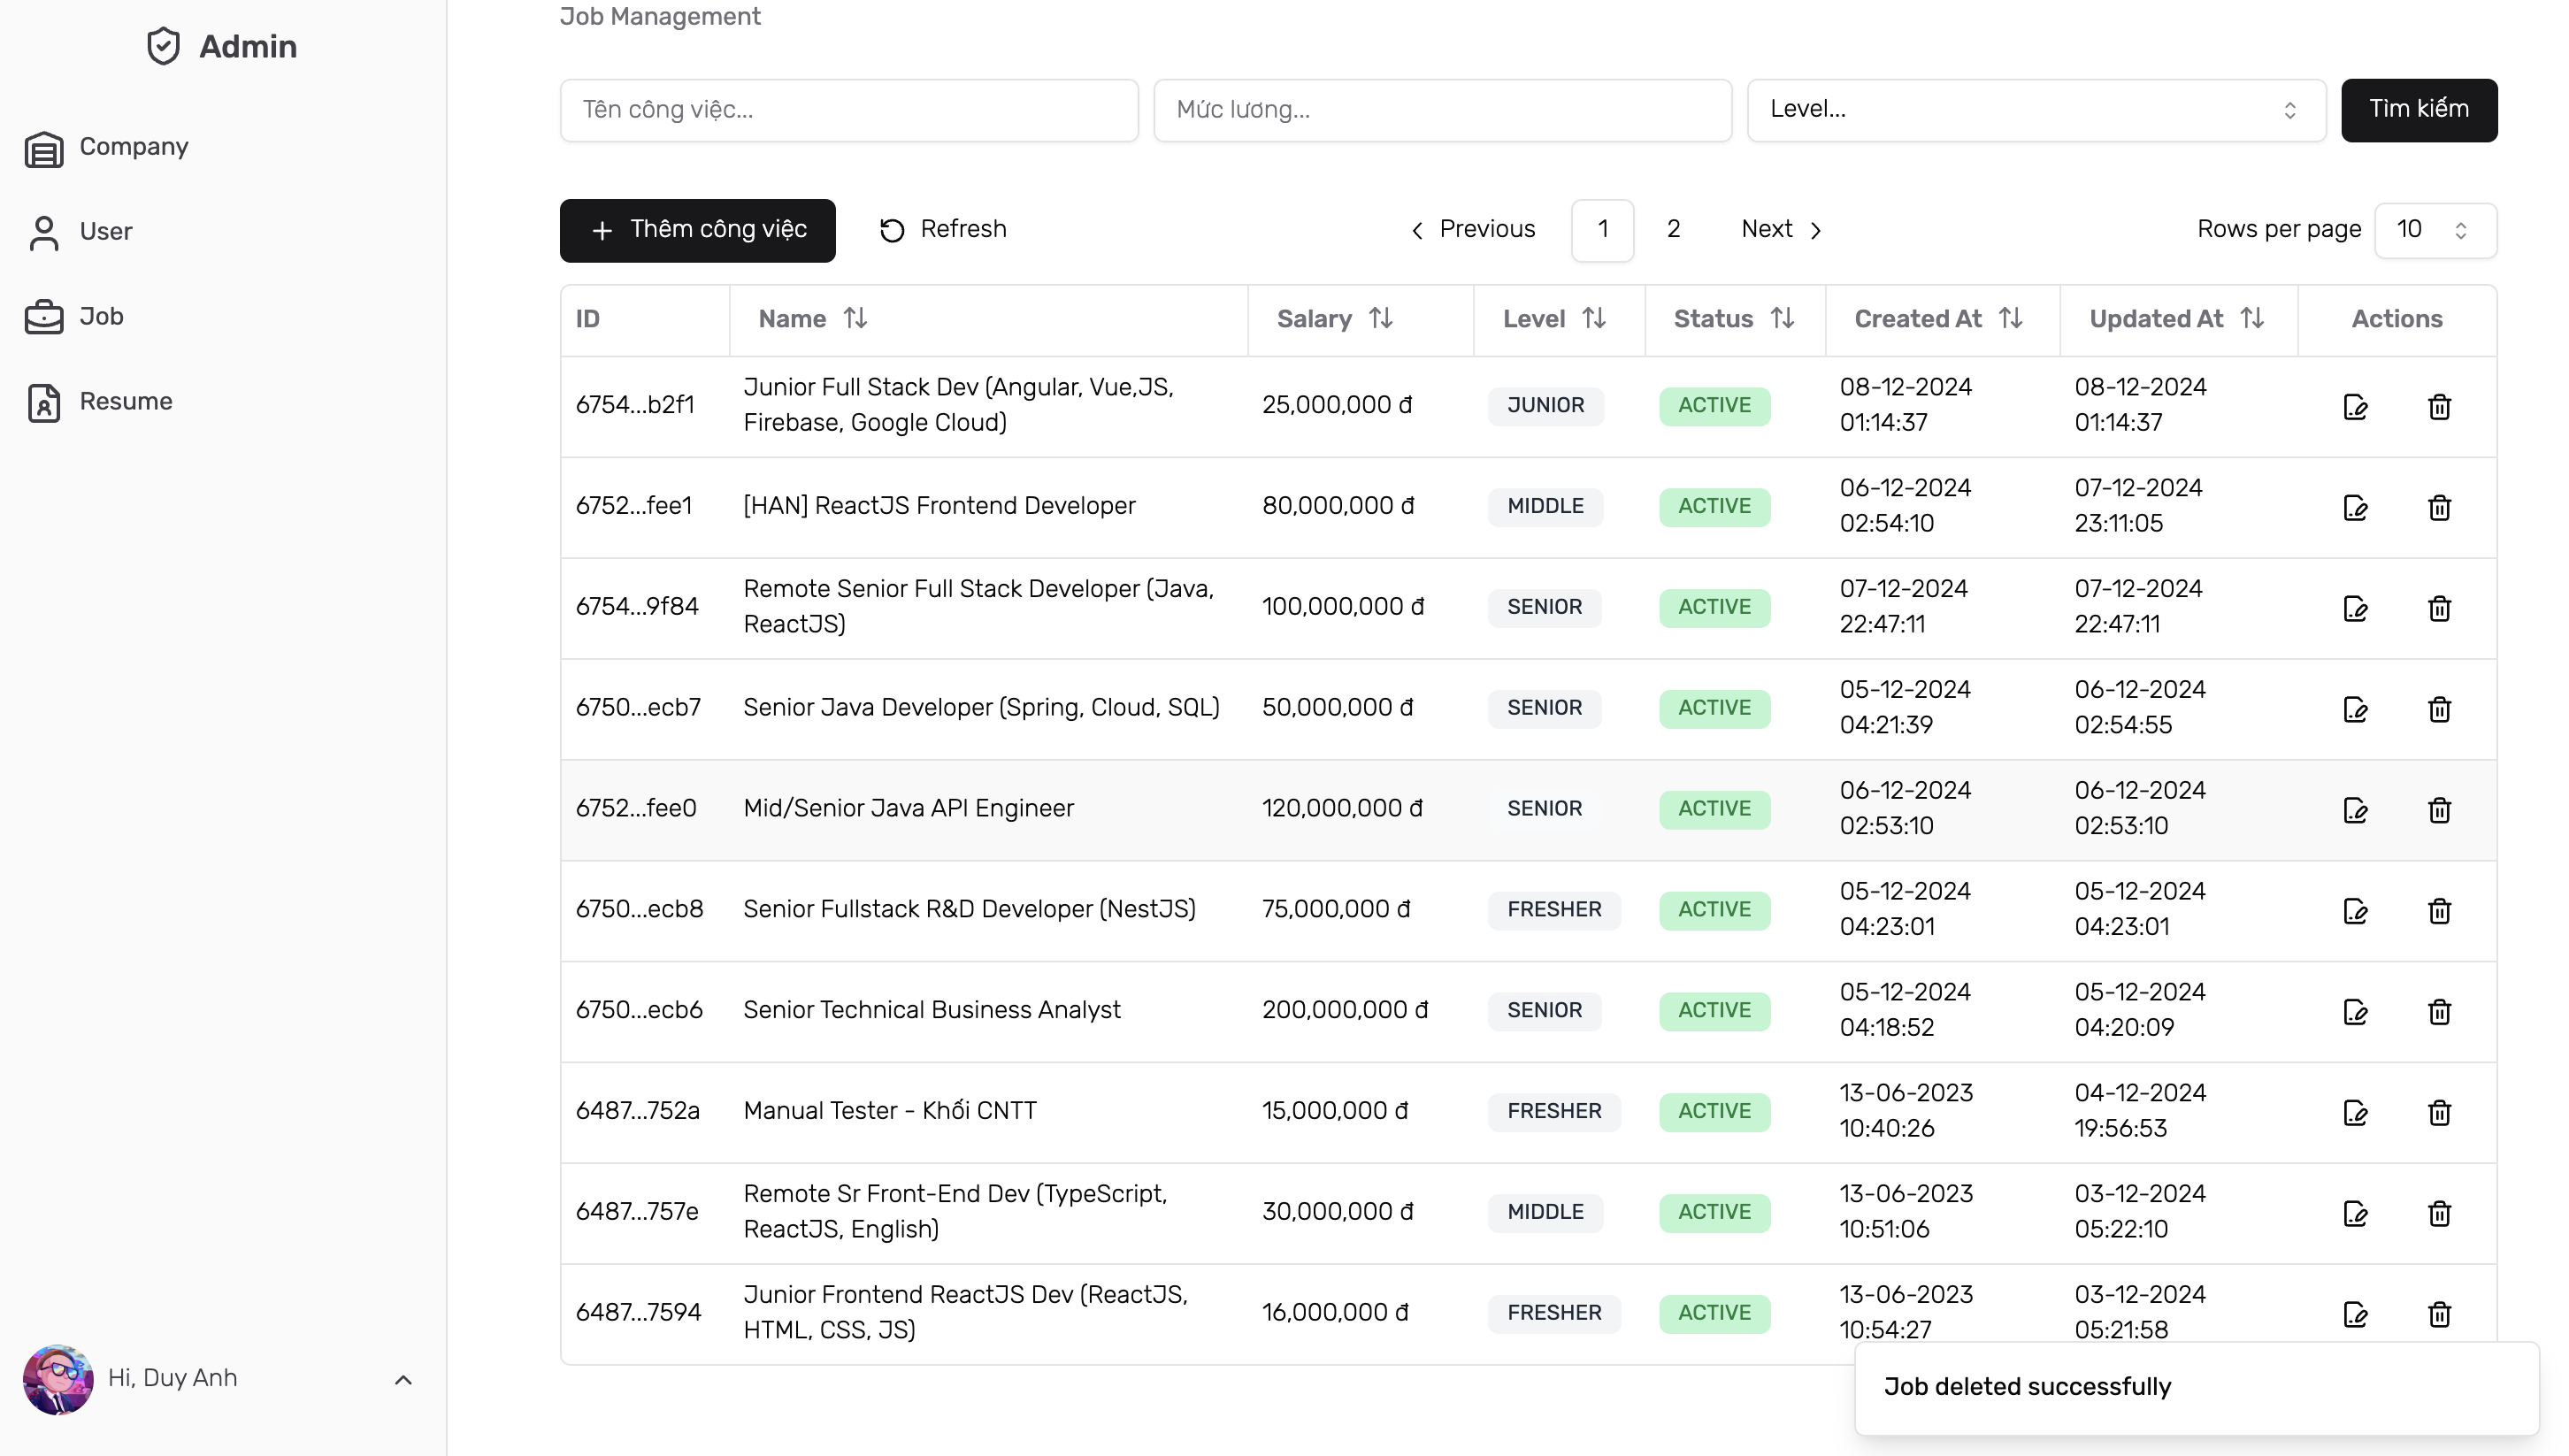
\includegraphics[width=\linewidth]{DBMS-Application/Images/delete-job-successfully.png}
    \caption{Trang quản lý công việc - Xoá thành công công việc đã chọn}
    \label{fig:enter-label}
\end{figure}

Truy vấn sử dụng: \textbf{Delete}

\begin{lstlisting}
const result = await this.db
      .collection('jobs')
      .deleteOne({ _id: new ObjectId(id) });
\end{lstlisting}